\section{Model}
\label{sec:model}

The formulation for treating pressurized cracks in a phase-field setting, first introduced by Hu~\cite{hu2021variationalthesis}, can be derived in two different ways.  In what follows, it is first derived based on energy minimization in quasi-static conditions in subsection \ref{qs_derivation}. This illustrates the main difference in the underlying hypothesis for this new model compared to the widely used formulations of \cite{bourdin2012variational} and \cite{mikelic2015quasi}, for example. A second derivation based on a maximum dissipation principle is then provided in subsection \ref{dyn_derivation}. 

The following assumptions are invoked for both derivations. A linear elastic body $\Omega \in \mathbb{R}^n$ ($n = 2$ or $3$), containing cracks denoted by $\Gamma$ is considered (Figure \ref{fig:potato}). The boundary $\partial\Omega$ is partitioned as $\partial\Omega = \partial\Omega_D \cup \partial\Omega_N$, where $\partial\Omega_D$ represents the portion of the boundary where displacements are prescribed and $\partial\Omega_N$ the portion where tractions are applied. Deformations and rotations are assumed to be small, so that a small-strain formulation is appropriate.  For simplicity, body forces are neglected.

\subsection{Quasi-static derivation}\label{qs_derivation}

\begin{figure}[ht]
    \centering
    \begin{tikzpicture}
        \node {\pgfimage[interpolate=false,width=.4\textwidth]{images/theory_part/potato_crack.png}};
        \draw (-0.1\textwidth,-0.1\textwidth) node {\LARGE$\Omega$};
        \draw (0.03\textwidth,0.03\textwidth) node {\LARGE\color{blue}$p$};
        \draw (0.075\textwidth,-0.05\textwidth) node {\LARGE$\Gamma$};
        \draw (0.16\textwidth,0.16\textwidth) node {\LARGE$\textbf{t}$};
    \end{tikzpicture}
    \caption{Generic body containing cracks loaded in pressure.}
    \label{fig:potato}
\end{figure}

The quasi-static derivation of the formulation begins by considering the potential energy of a body with cracks which are internally loaded with a pressure $p$.  Crack propagation is associated with a critical fracture energy density, $G_c$.  The total potential energy is given by
\begin{equation}\label{total potential static}
    U(\bs{\epsilon}(\textbf{u})) = \int\limits_{\Omega}\psi_e(\bs\epsilon(\textbf{u}))\ \text{dV} + \int\limits_{\Gamma} G_c \, \text{dA} - \int\limits_{\Gamma} p\textbf{n}\cdot\textbf{u}\ \text{dA} - \int\limits_{\partial \Omega_N} \textbf{t}\cdot\textbf{u} \ \text{dA},
\end{equation}
in which $\textbf{u}$ are the displacements, $\bs \epsilon(\textbf{u}) = \nabla^s\textbf{u}$ denotes the infinitesimal strain, $\psi_e$ the strain energy density, $\textbf{t}$ the externally applied tractions and $\textbf{n}$ the unit normals of the crack set $\Gamma$ (oriented outwards from $\Omega$).  

In a phase-field for fracture setting, the crack surface $\Gamma$ is regularized with the aid of a scalar phase (or damage) field $d ({\bf{x}}) \in[0,1]$.  In this work, $d = 0$  represents intact material (away from the crack surface) and $d=1$ fully-damaged material (inside the crack).  The damage field is employed in the approximation of the surface integrals in \eqref{total potential static} as volume integrals.  For the energy associated with fracture, several common formulations are encapsulated by the approximation
\begin{equation}
    \int\limits_{\Gamma} G_c \, dA \approx  \int\limits_{\Omega} \dfrac{G_c}{c_0\ell}\bigg( \alpha(d) + \ell^2\nabla d \cdot \nabla d\bigg)\ \text{dV}, 
\end{equation}
where $\alpha(d)$ denotes a local dissipation term, $\ell$ is the regularization length, and $c_0$ is a normalization constant given by $c_0 = 4\int_0^1\sqrt{\alpha(s)}ds$.

Such a regularization implies that the distinct crack surface $\Gamma$ is no longer defined.  As such, the second integral on the right of \eqref{total potential static} also needs to be approximated as a volume integral in some manner.  This is effected with the use of an indicator function $I(d)$.  The surface integral involving the pressure is then approximated as
\begin{equation}\label{reg pressure term}
    \int\limits_{\Gamma} p\textbf{n}\cdot{\textbf{u}} \text{dA} \approx \int\limits_{\Omega} p \left( -\frac{\nabla d}{\Vert\nabla d\Vert} \right)\cdot{\textbf{u}} \Vert\nabla I(d)\Vert\text{dV}.
\end{equation}
Note that the crack surface normal $\textbf{n}$ is approximated as $-{\nabla d}/{\Vert\nabla d\Vert}$, whereas the differential surface element $\text{dA}$ becomes $\Vert\nabla I\Vert\text{dV}$.  The indicator function must satisfy $I(0)=0$, $I(1)=1$ and be monotonically increasing. In Bourdin et al.~\cite{bourdin2012variational}, $I(d)=d$ was firstly proposed. Wheeler et al.~\cite{wheeler2014augmented} provide a derivation that avoids an explicit approximation of the normal, such as \eqref{reg pressure term}, but is in fact equivalent to using the indicator function $I(d) = 2d - d^2$. In Peco et al.~\cite{peco2017influence} and Jiang et al.~\cite{jiang2022phase}, $I(d) = d^2$ is used, with the motivation that $I'(0) = 0$ is required to avoid the effects of pressure in undamaged areas.

Combining the approximation in \eqref{reg pressure term} with the traditional phase-field approximation of fracture based on the Ambrosio-Tortorelli functional \cite{bourdin2000numerical} and applying the chain rule, the regularized counterpart of \eqref{total potential static} is given by
\begin{multline}\label{total potential static pf}
    U(\bs{\epsilon},d) = \int\limits_{\Omega}\psi_e(\bs\epsilon,d)\ \text{dV} + \int\limits_{\Omega} p \nabla d\cdot\textbf{u}\ I'(d)\text{dV} \\ + \int\limits_{\Omega}\dfrac{G_c}{c_0\ell}\bigg( \alpha(d) + \ell^2\nabla d \cdot \nabla d\bigg)\ \text{dV} - \int\limits_{\partial \Omega_N} \textbf{t}\cdot\textbf{u} \ \text{dA},
\end{multline}
where the explicit dependence of the strain on the displacements has been dropped.  

Often, the strain energy density is split and part of it is degraded with the damage, i.e. 
\begin{equation}\label{energy split}
    \psi_e(\bs\epsilon(\textbf{u}),d) = g(d)\psi^+_e(\bs\epsilon(\textbf{u})) + \psi_e^-(\bs\epsilon(\textbf{u})),
\end{equation}
where $g(d)$ denotes the degradation function, and $\psi_e^+(\bs\epsilon(\textbf{u}))$ and $\psi_e^-(\bs\epsilon(\textbf{u}))$ denote the ``active" and ``inactive" parts of the energy. The above form encapsulates most of the strain decompositions used in the literature \cite{amor2009regularized},\cite{miehe2010phase} to introduce asymmetry in the fracture behavior in tension and compression.

Typically, a minimization principle is applied to \eqref{total potential static pf} to extract the governing equations for the displacements $\textbf{u}$ and the damage $d$. According to this principle, a pair ($\textbf{u}$, $d$) is a valid state if and only if all neighboring states ($\textbf{u} + \delta\textbf{u} $, $d+\delta d$) have a greater potential energy. In the case of pressurized cracks, a subtle consideration leads to the formulation proposed herein. Consider the two scenarios indicated in Figure \ref{fig:wet_vs_dry_crack}. In the situation depicted in Figure \ref{fig:wet_crack}, the pressure load (applied in the areas colored in blue), is assumed to accompany any crack propagation. Therefore, in an energetic analysis, the virtual crack extension $da$ is assumed  pressurized. By contrast, in Figure \ref{fig:dry_crack}, the pressure load is assumed to remain confined to the original crack geometry during propagation.  As a result, the virtual crack extension $da$ is not subject to any surface load.

In terms of the resulting formulation, the difference between the two scenarios shown in Figure \ref{fig:wet_vs_dry_crack} translate into the question of whether or not the damage variation $\delta d$ should enter the pressure work contribution \eqref{reg pressure term}.

For the family of formulations that derived from \cite{bourdin2012variational} and \cite{wheeler2014augmented}, the scenario depicted in Figure \ref{fig:wet_crack} is assumed as a consequence of including the damage variation $\delta d$ in \eqref{reg pressure term}. The proposed model in this work, by contrast, assumes the case indicated by Figure \ref{fig:dry_crack}.  Although these competing views are expected to give rise to negligible differences in results in the limit as $da \rightarrow 0$, in practice the two formulations do give rise to slightly different sets of governing equations.  As we will demonstrate in the numerical examples in Section~\ref{sec:results}, in practice these differences can translate into fairly significant differences in the results.  

\begin{figure}[h]
% \centering
\bigskip
\begin{subfigure}{.49\textwidth}
  \centering
  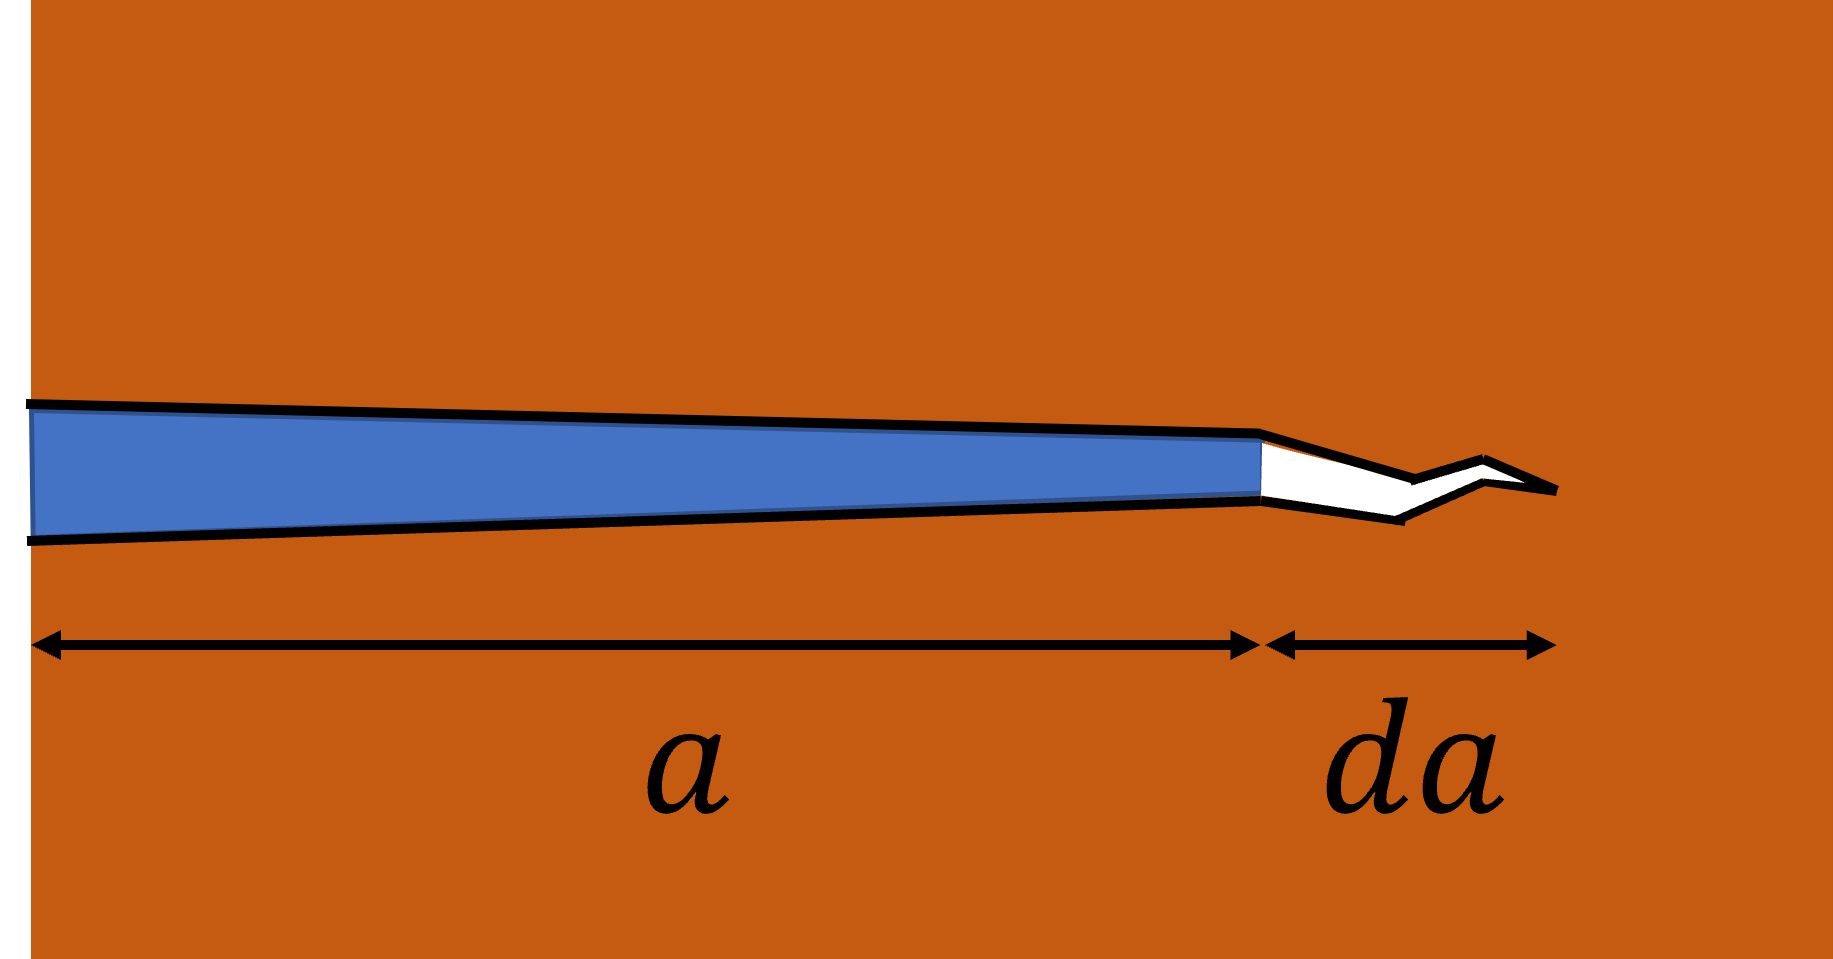
\includegraphics[width=0.7\linewidth]{images/theory_part/dry_crack.png}
  \caption{}
  \label{fig:dry_crack}
\end{subfigure}%
\begin{subfigure}{.49\textwidth}
  \centering
  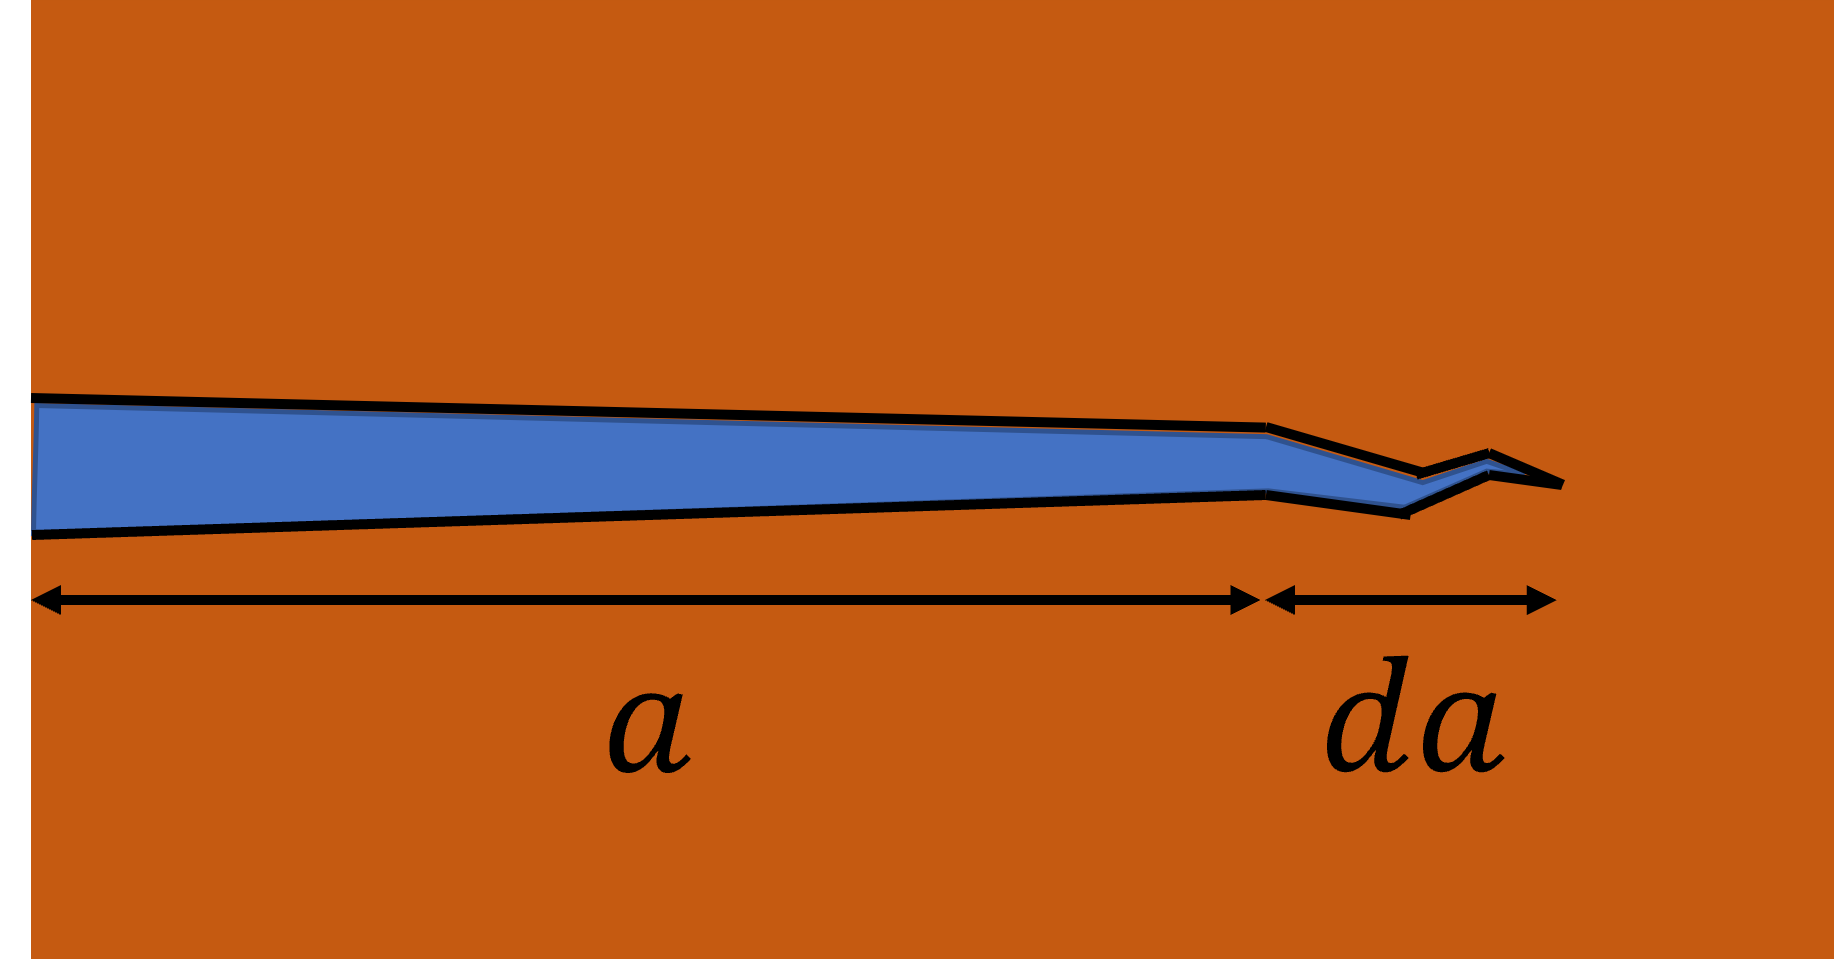
\includegraphics[width=0.7\linewidth]{images/theory_part/wet_crack.png}
  \caption{}
  \label{fig:wet_crack}
\end{subfigure}%
  \caption{(a) Unloaded virtual crack. (b) Pressure loaded virtual crack;} 
  \label{fig:wet_vs_dry_crack}
\end{figure}

In what follows, the formulation associated with Figure \ref{fig:dry_crack} will be referred to as the Unloaded Virtual Crack formulation, or UVC for short. In the UVC, the variation of the pressure work is simply\footnote{\noindent On the other hand, if the assumption of Figure \ref{fig:wet_crack} is chosen, as in \cite{bourdin2012variational}, two additional terms have to be accounted for, \begin{equation*}\label{wet variation}
    \delta \left( \int\limits_{\Omega} p \nabla d\cdot\textbf{u}\ I'(d)\text{dV} \right) = \int\limits_{\Omega} p \nabla d\cdot\delta\textbf{u}\ I'(d)\text{dV} \underbrace{+ \int\limits_{\Omega} p \nabla \delta d\cdot\textbf{u}\ I'(d)\text{dV} + \int\limits_{\Omega} p \nabla d\cdot\textbf{u}\ \delta d\ I''(d)\text{dV}}_{\text{additional terms}}.
\end{equation*}},

\begin{equation}\label{dry variation}
    \delta \left( \int\limits_{\Omega} p \nabla d\cdot\textbf{u}\ I'(d)\text{dV} \right) = \int\limits_{\Omega} p \nabla d\cdot\delta\textbf{u}\ I'(d)\text{dV}.
\end{equation}

\noindent The variation of the potential energy $\delta U$ can then be written as,

\begin{multline}
    \delta U(\bs{\epsilon},d) = \int\limits_{\Omega}\dfrac{\partial\psi_e}{\partial \bs \epsilon}:\delta\bs\epsilon\ \text{dV} + \int\limits_{\Omega} p \nabla d\cdot\delta\textbf{u}I'(d)\ \text{dV} 
    - \int\limits_{\partial \Omega_N} \textbf{t}\cdot\delta\textbf{u} \ \text{dA} \\
    + \int\limits_{\Omega}g'(d) \psi_e^+(\bs\epsilon)\delta d\ \text{dV}
    + \int\limits_{\Omega}\dfrac{G_c}{c_0\ell}\bigg( \alpha'(d)\delta d + 2\ell^2\nabla d \cdot \nabla \delta d\bigg)\ \text{dV},
\end{multline}

and, with the help of the divergence theorem, 

\begin{align}
    \delta U(\bs{\epsilon},d) =& \int\limits_{\Omega}\biggl(-\nabla \cdot \dfrac{\partial\psi_e}{\partial \bs \epsilon} + pI'(d) \nabla d\biggr)\cdot\delta\textbf{u}\ \text{dV} 
    + \int\limits_{\partial \Omega_N}\biggl( \dfrac{\partial\psi_e}{\partial \bs \epsilon}\cdot\textbf{n}  -\textbf{t}\biggr)\cdot\delta\textbf{u} \ \text{dA} \\
    +& \int\limits_{\Omega}\left(g'(d) \psi_e^+(\bs\epsilon)
    + \dfrac{G_c}{c_0\ell}\alpha'(d) - \nabla \cdot\dfrac{2G_c\ell}{c_0}\nabla d \right)\delta d\ \text{dV} + \int\limits_{\partial\Omega} \dfrac{2G_c\ell}{c_0}(\textbf{n}\cdot\nabla d)  \delta d\ \text{dA}.
\end{align}

The local minimization principle requires the variation of the potential energy $\delta U$ to be non-negative for any admissible state $\textbf{u},d$. In other words, $\delta U(\bs\epsilon, d) \ge 0$, giving rise to the following equation and boundary condition for $\textbf{u}$, since the variation of the displacement field $\delta \textbf{u}$ is arbitrary:

\begin{equation}\label{disp equation}
    -\nabla \cdot \bs \sigma  + pI'(d) \nabla d = 0 \text{ on }\Omega,
\end{equation}

\begin{equation}\label{disp bcs}
    \bs\sigma \cdot \textbf{n} - \textbf{t} = 0 \text{ on }\partial\Omega_N.
\end{equation}

\noindent In the above, $\bs\sigma$ denotes the Cauchy stress, defined as $\bs\sigma = \dfrac{\partial\psi_e}{\partial \bs \epsilon}$. 

For the damage variable, it is assumed that the process is irreversible, such that $\dot{d} \ge 0$.  As such, only positive variations in the damage are admissible, and $\delta U(\bs\epsilon, d) \ge 0$ implies

\begin{equation}\label{damage equation}
    g'(d) \psi_e^+(\bs\epsilon)
    + \dfrac{G_c}{c_0\ell}\alpha'(d) - \nabla \cdot \dfrac{2G_c\ell}{c_0}\nabla d \ge 0 \text{ on }\Omega,
\end{equation}
\begin{equation}\label{damage bcs}
    \dfrac{2G_c\ell}{c_0}\textbf{n}\cdot \nabla d \ge 0 \text{ on }\partial\Omega.
\end{equation}

\noindent Equations \eqref{damage equation} and \eqref{damage bcs} are identical to those in the standard phase-field model for traction-free cracks. This is the main difference between the new formulation and existing ones derived from deriving from \cite{bourdin2012variational} and \cite{wheeler2014augmented}, in which the governing equation for the damage field contains additional terms to account for the pressure loads on the virtual cracks. In what follows, we refer to that as the Loaded Virtual Crack formulation, or LVC.  In the boxes below, the governing equations for the UVC are compared to those of the LVC.  

\bigskip
\noindent
\begin{mdframed}[
    frametitle={\begin{equation}\label{uvc}\tag{UVC}\text{Unloaded Virtual Crack Formulation}\end{equation}},
    frametitlebackgroundcolor=gray!20,
    backgroundcolor=gray!5,
    linewidth=0pt,
    nobreak=true
  ]
  
\begin{equation}\label{disp equation box}
    -\nabla \cdot \bs\sigma  + pI'(d) \nabla d = 0 \text{ on }\Omega,
\end{equation}

\begin{equation}\label{disp bcs box}
    \bs\sigma\cdot \textbf{n} -\textbf{t} = 0 \text{ on }\partial\Omega_N.
\end{equation}

\begin{equation}\label{damage equation box}
    g'(d) \psi_e^+(\bs\epsilon)
    + \dfrac{G_c}{c_0\ell}\alpha'(d) - \nabla \cdot \dfrac{2G_c\ell}{c_0}\nabla d \ge 0 \text{ on }\Omega,
\end{equation}

\begin{equation}\label{damage bcs box}
    \dfrac{2G_c\ell}{c_0}\textbf{n}\cdot \nabla d \ge 0 \text{ on }\partial\Omega.
\end{equation}
  
\end{mdframed}
%\end{minipage}
\hspace{.03\linewidth}
%\begin{minipage}{.48\linewidth}
\begin{mdframed}[
    frametitle={\begin{equation}\label{lvc}\tag{LVC}\text{Loaded Virtual Crack Formulation}\end{equation}},
    frametitlebackgroundcolor=gray!20,
    backgroundcolor=gray!5,
    linewidth=0pt,
    nobreak=true
  ]
  
\begin{equation}\label{disp equation box2}
    -\nabla \cdot \bs\sigma  + pI'(d) \nabla d = 0 \text{ on }\Omega,
\end{equation}

\begin{equation}\label{disp bcs box2}
    \bs\sigma\cdot \textbf{n} - \textbf{t} = 0 \text{ on }\partial\Omega_N.
\end{equation}

\begin{multline}\label{wet damage equation box2}
    g'(d) \psi_e^+(\bs\epsilon)
    + \dfrac{G_c}{c_0\ell}\alpha'(d) - \nabla \cdot \dfrac{2G_c\ell}{c_0}\nabla d \\ - \nabla \cdot [p\textbf{u}\ I'(d)] + p\nabla d\cdot \textbf{u}I''(d) \ge 0 \text{ on }\Omega,
\end{multline}
    
\begin{equation}\label{wet damage bcs box2}
    \textbf{n}\cdot \left(\dfrac{2G_c\ell}{c_0}\nabla d+   pI'(d)\textbf{u}\right) \ge 0 \text{ on }\partial\Omega.
\end{equation}
  
\end{mdframed}

\noindent It is readily apparent that the governing equations for the displacements are identical in the UVC and the LVC. The main difference is in the absence of the additional pressure-dependent terms in the evolution for the damage field and the accompanying boundary condition.  

In \ref{SIF_equivalence}, an analytical study of the energy release rate of a crack propagating under an arbitrary pressure load $p(x)$ is provided, under the assumptions of the UVC formulation and linear elastic fracture mechanics. The results of the study show that it is possible to recover the classic relationship between the energy release rate and the stress intensity factor with the UVC formulation. This ensures the consistency of the proposed formulation \eqref{uvc} with many theoretical works \cite{detournay2016mechanics, garagash2000tip, detournay2004propagation, garagash2005plane, bunger2005toughness} in the field of hydraulic fracture, where the stress intensity factor is used as the propagation criteria

\subsection{Derivation using the maximum dissipation principle}\label{dyn_derivation}

In this subsection, an alternative approach to derive the \eqref{uvc} formulation  is presented. It is based on the construction of a total potential functional which depends on the rates of the internal variables $\dot{\bs\epsilon},\dot{d}$ and accounts for  the work of the pressure load as an external dissipation mechanism. This approach is described in more detail in \cite{hu2021variationalpaper} and \cite{hu2021variationalthesis}, where it is used to derive a variationally consistent phase-field model for ductile fracture. 

The total potential is postulated as,

\begin{equation}\label{total potential}
    L(\dot{\bs\epsilon},\dot{d}) = \int\limits_{\Omega} \dot{u}(\dot{\bs\epsilon},\dot{d}) \text{dV} - \mathcal{P}^{ext}, 
\end{equation}
where $u$ is the material internal energy, which relates to the Helmholtz free-energy $\psi$ through $\dot{u} = \dot{\psi} + \dot{T}s$, where $T$ is the temperature and $s$ the entropy. 
In this work, only isothermal processes are considered, therefore, $\dot{u} = \dot{\psi}$. The term $\mathcal{P}^{ext}$ denotes the external power expenditure. If cracks were represented by internal boundaries $\Gamma$ instead of a damage field, one could write,

\begin{equation}\label{power expenditure}
    \mathcal{P}^{ext} = \int\limits_{\partial \Omega \cup \Gamma} \textbf{t}\cdot\dot{\textbf{u}} \text{dA} = \int\limits_{\partial \Omega} \textbf{t}\cdot\dot{\textbf{u}} + \int\limits_{\Gamma} p\textbf{n}\cdot\dot{\textbf{u}} \text{dA}.
\end{equation}

\noindent However, in a regularized setting this integral over $\Gamma$ is once again transformed into a volume integral over $\Omega$, as in \eqref{reg pressure term}, 

\begin{equation}\label{reg power expenditure}
    \int\limits_{\Gamma} p\textbf{n}\cdot\dot{\textbf{u}} \text{dA} \approx \int\limits_{\Omega} p \left( -\frac{\nabla d}{\Vert\nabla d\Vert} \right)\cdot\dot{\textbf{u}} \Vert\nabla I(d)\Vert\text{dV} = 
    -\int\limits_{\Omega}p\nabla d \cdot\dot{\textbf{u}} I'(d) \text{dV}.
\end{equation}

Recalling the equivalence between the internal energy and the Helmholtz free-energy, the Coleman-Noll procedure can be applied and, in combination with \eqref{power expenditure} and \eqref{reg power expenditure}, leads to the following expression for $L$ as a function of $\psi$: 

\begin{equation}
    L(\dot{\bs\epsilon},\dot{d}) = \int\limits_{\Omega} \left( \dfrac{\partial\psi}{\partial\bs\epsilon}:\dot{\bs\epsilon} + \dfrac{\partial\psi}{\partial d}\dot{d}+\dfrac{\partial\psi}{\partial \nabla d}\cdot {\nabla \dot d} + p\nabla d \cdot\dot{\textbf{u}} I'(d) \right) \text{dV} - \int\limits_{\partial \Omega} \textbf{t}\cdot\dot{\textbf{u}} \text{dA}. 
\end{equation}

The evolution process is postulated to follow the minimizers of this total potential, with the supplemental conditions that damage is an irreversible process and that the displacements $\textbf{u}$ are prescribed over a subset $\partial \Omega_D$ of the boundary. In other words, 

\begin{equation}\label{minimization principle}
    \dot{\bs\epsilon}, \dot{d} = \underset{\dot{\bs\epsilon},\dot{d}}{{\operatorname{argmin}}} \ L(\dot{\bs\epsilon}, \dot{d}) \text{,\ \   subject to } \dot{d} \ge 0 \text{ and } \textbf{u}=\textbf{g} \text{ on }\partial \Omega_D. 
\end{equation}

\noindent Using the Euler-Lagrange equations, the following general evolution equations can then be obtained in terms of the free-energy function $\psi$:
\begin{equation}\label{u_equation}
    \nabla \cdot \dfrac{\partial\psi}{\partial \bs\epsilon} - pI'(d) \nabla d = 0 \text{ on }\Omega,
\end{equation}
\begin{equation}\label{d_equation}
    \nabla \cdot \dfrac{\partial\psi}{\partial \nabla d} - \dfrac{\partial\psi}{\partial d} \ge 0 \text{ on }\Omega,
\end{equation}
with the boundary conditions
\begin{equation}\label{u_bc_helmholtz}
    \dfrac{\partial\psi}{\partial \bs\epsilon}\cdot\textbf{n} - \textbf{t} = 0 \text{ on }\partial\Omega\setminus\partial\Omega_D
\end{equation}
\begin{equation}\label{d_bc_helmholtz}
    \textbf{n} \cdot \dfrac{\partial\psi}{\partial \nabla d} \ge 0 \text{ on }\partial\Omega.
\end{equation}

\noindent To be consistent with the derivation in subsection \ref{qs_derivation}, the Helmholtz free-energy is postulated as,

\begin{equation}\label{helmholtz free-energy postulate}
    \psi(\bs{\epsilon},d) = \psi_e(\bs{\epsilon},d) + \dfrac{G_c}{c_0\ell}\bigg( \alpha(d) + \ell^2\nabla d \cdot \nabla d\bigg),
\end{equation}

\noindent following the regularization based on the Ambrosio-Tortorelli functional. In this case, the general equations \eqref{u_equation}-\eqref{d_bc_helmholtz} take the form
\begin{equation}
\label{eq:UVC-eq2}
    -\nabla \cdot \bs\sigma  + pI'(d) \nabla d = 0 \text{ on }\Omega,
\end{equation}
\begin{equation}
    g'(d) \psi_e^+(\bs\epsilon)
    + \dfrac{G_c}{c_0\ell}\alpha'(d) - \nabla \cdot \dfrac{2G_c\ell}{c_0}\nabla d \ge 0 \text{ on }\Omega,
\end{equation}
 with the boundary conditions
\begin{equation}
    \bs\sigma\cdot \textbf{n}-\textbf{t} = 0 \text{ on }\partial\Omega_N,
\end{equation}
\begin{equation}
\label{eq:UVC-bc2}
    \textbf{n}\cdot \nabla d \ge 0 \text{ on }\partial\Omega.
\end{equation}
By inspection, \eqref{eq:UVC-eq2}-\eqref{eq:UVC-bc2} are identical to \eqref{disp equation}-\eqref{damage bcs}.

\subsection{Constitutive choices of the phase-field formulation}

In the previous subsection, the proposed model for pressurized cracks was developed for a general phase-field regularization of the variational approach to fracture \cite{francfort1998revisiting}, with a free-energy of the form

\begin{equation}\label{PF general form}
    \psi(\bs{\epsilon},d) = \underbrace{g(d)\psi_e^+(\bs{\epsilon}) + \psi_e^-(\bs{\epsilon})}_{\psi_e} + \underbrace{\frac{G_c}{c_0\ell}\bigg( \alpha(d) + \ell^2\nabla d \cdot \nabla d\bigg)}_{\psi_f}.
\end{equation}

\noindent In what follows, the constitutive choices used in the example problems provided in Section \ref{sec:results} are described. 

\subsubsection{Elastic energy and decomposition}

First, in terms of the solid bulk response, an elastic energy of the type \eqref{energy split} is assumed. When the material is undamaged, it reduces to a purely linear elastic energy, that is,

\begin{equation}
    \psi_e(\bs\epsilon(\textbf{u}),0) = \psi_e^+(\bs\epsilon(\textbf{u}),0)+\psi_e^-(\bs\epsilon(\textbf{u}),0) = \dfrac{1}{2}\bs\epsilon(\textbf{u}) : \mathbb{C} : \bs\epsilon(\textbf{u}),
\end{equation}

\noindent where $\mathbb{C}$ is the elasticity tensor.

When damage is present, a decomposition of the energy is often assumed. In many cases, when the applied load to a fracturing body is predominately tensile, the ``no-split" case given by,

\begin{equation}
    \psi_e^-(\bs\epsilon(\textbf{u}),d)=0 \rightarrow \psi_e(\bs\epsilon(\textbf{u}),d) = \dfrac{1}{2}g(d)\bs\epsilon(\textbf{u}) : \mathbb{C} : \bs\epsilon(\textbf{u}),
\end{equation}

\noindent is capable of correctly predicting the material response, while leading to a simpler set of governing equations. However, in a wide-range of scenarios, compressive forces are present, and an energy split is needed to prevent crack formation in zones of high compression, as well as to allow for transmission of compressive forces across fractured faces. 

In Section \ref{sec:results}, one of the example problems will employ the spectral split of Miehe et al. \cite{miehe2010phase},  given by,

\begin{equation}
    \psi_e^+(\bs\epsilon(\textbf{u}),d) = \dfrac{1}{2}\lambda\left<\text{Tr }\bs\epsilon\right>_+^2+\mu\bs\epsilon^+:\bs\epsilon^+ \text{ and }  \psi_e^-(\bs\epsilon(\textbf{u}),d) = \dfrac{1}{2}\lambda\left<\text{Tr }\bs\epsilon\right>_-^2+\mu\bs\epsilon^-:\bs\epsilon^-.
\end{equation}

Here, $\left< \cdot \right>_+$ and $\left< \cdot \right>_-$ denote the positive and negative parts of a number respectively, while $\bs\epsilon^+$ and $\bs\epsilon^-$ are the positive and negative parts of an additive decomposition of the strain tensor based on the signs of its eigenvalues. A more detailed description, including the derivation of the stiffness matrix in this case, is provided by Jiang et al.\ \cite{jiang2020three}.

\subsubsection{Brittle fracture}

The first and more traditional phase-field model with an energy of the type \eqref{PF general form} was proposed in \cite{bourdin2000numerical}. It was developed to approximate the brittle fracture process of linear elastic materials in the limit of vanishing $\ell$. In its original form, the degradation function 

\begin{equation}\label{quadratic_degradation}
    g(d) = \xi + (1-\xi)(1-d)^2,
\end{equation}

\noindent is used in combination with a quadratic local dissipation $\alpha(d) = d^2$, in what is now called the AT-2 formulation. However, the use of, $\alpha(d) = d$, (widely referred as the AT-1) comes with the advantage of a purely elastic response before the onset of damage and a compactly supported damage field. Therefore, it will be employed in the example in Section \ref{sec:results} where brittle fracture is investigated. The parameter $\xi$ in \eqref{quadratic_degradation} is the residual stiffness, a very small numerical parameter that avoids the loss of ellipticity in fully damaged material.

\subsubsection{Cohesive fracture}\label{cohesive_frac}

The phase-field model for cohesive fracture was first proposed by Lorentz et al. \cite{lorentz2011convergence, lorentz2011gradient}. In this model, the use of a quasi-quadratic degradation function, given by
\begin{equation}\label{cohesive_degradation}
    g(d) = \xi + (1-\xi)\dfrac{(1-d)^2}{(1-d)^2+md(1+pd)},
\end{equation}
is combined with a linear local dissipation function $\alpha(d) = d$.  The parameter $m$ is defined as $m = \dfrac{G_c}{c_0\ell\psi_c}$, where $\psi_c$ is the nucleation energy, below which no damage is expected to form.  The parameter $p$ is a shape parameter that can be used to adjust the traction-separation response.  In this work, $p=1$ is used.  